\subsubsection{Protocolo de Comunicação via Rádio Frequência}

O protocolo utilizado no link de rádio frequência criado será o MAVLink - \textit{Micro Air Vehicle Message Marshalling Library} - é uma biblioteca de comunicação para 
pequenas quantidades de dados entre aeronaves não tripuladas e estações de controle em terra. 
Permitindo o envio de pacotes de informações através de \textit{byte-level serialization} o que torna 
compatível com qualquer onda de radio.\cite{mavlink}

Uma vez que a área de atuação do EmerVant é a Esplanada dos Ministérios, 
definido na seção \ref{escopo} - Escopo, a viabilidade e eficiência na implantação desse protocolo é
extremamente alta. Aonde o sinal emissor será posicionado na torre de TV cobrindo toda a 
área de atuação com um boa qualidade de sinal. 

\subsubsection{Especificação do Projeto da Comunicação do Vant}

A comunicação entre a central de atendimento, responsável por receber a chamada de emergência, e a central de controle, responsável pelo controle, comando e monitoramento do VANT, ocorrerá da seguinte forma:

\begin{itemize}
  \item A central de atendimento recebe a chamada de emergência.
  \item Verifica a necessidade de enviar o VANT. Analisando o tempo hábil para a chegada da ambulância.
  \item Caso necessário, a ambulância  ligará para a central de controle, para que a mesma envie o VANT para o local indicado.
  \item A partir da decolagem do VANT, a comunicação passa a ocorrer via RF(radiofreqüência) com a central de controle.
  \item Quando o VANT chegar ao local, o controlador instrui o usuário à usar o desfibrilador na vitima, se necessário. Tal comunicação é feita por RF.
  \item Após o atendimento, a ambulância que já terá se dirigido ao local de atendimento, para a finalização do atendimento e o encaminhamento da vitima para o hospital, ela recolherá o VANT.
 
\end{itemize}

\begin{itemize}
 \item Piloto automático guiará o VANT até a emergência: 

  A central receberá a solicitação do veículo e com as orientações do local do acidente, ela irá mapear o percurso a ser seguido para chegar até o destino.  Essas informações referentes ao trajeto e coordenadas de GPS serão passadas de forma wireless serialmente para o sistema e controladores do VANT. Para que isso aconteça, eles estarão conectadas por um canal de comunicação de radiofrequência. 

  \item Comunicação e transmissão de dados:

   A central necessitará passar informações ao usuário referentes ao atendimento, também precisará ver o estado do paciente e ver se os procedimentos foram realizados conforme as instruções e as informações dos sinais vitais da vítima para entender a real situação dele. 
\end{itemize}
\subsubsubsection{Comunicação com o Pixhawk}
O controle e configura\c{c}\~ao do voo do VANT \'e gerenciado pelo \textit{Ground Control Station}, em português, 
esta\c{c}\~ao de controle em solo. Inicialmente seria desenvolvido um sistema que atendesse os requisitos levantados no Documento
de Visão do Projeto (em anexo), todavia com a pesquisa de sistemas existentes concorrentes optou-se por utilizar o \textit{software Mission Planner}. 
Devido à facilidade na customização e a compatibilidade com a placa controladora adotada 
pelo projeto, Pixhawk, esse sistema é mantido pelo projeto \textit{open-source  APM autopilot}.\cite{gcs}

Foram analisados os seguintes \textit{softwares} e essa análise pode ser vista na Figura \ref{fig:gcstable}: 

\begin{itemize}
  \item QGroundControl
  \item Mission Planner
  \item APMPlanner
\end{itemize}
\pagebreak
\begin{figure}[H]
    \centering
      \includegraphics[keepaspectratio=true,scale=0.45]{figuras/gcstable.eps}
    \caption{Resultado da análise dos softwares de GCS.}
    \label{fig:gcstable}
\end{figure}

\pagebreak
Pela Figura \ref{fig:gcstable}, pode-se perceber que o software Mission Planner é a melhor solução para o gerênciamento do VANT. Uma vez que o projeto está sob uma licença aonde é permitido o uso para comercialização, este será utilizado com GCS do VANT.

Com a utilização do \textit{GCS Mission Planner}, o processo da operação de socorro é automatizado. 
Uma vez que, com a aplicação é possível a criação de planos de voos. 
A figura \ref{fig:planovoo} mostra um exemplo de plano de voo. 
Nesse plano, o VANT decola do ponto \textit{Home}, em seguida é direcionado até ao ponto 2 e depois 
se desloca ao ponto 3 e retorna ao ponto inicial.

\begin{figure}[H]
    \centering
	    \includegraphics[keepaspectratio=true,scale=0.5]{figuras/planovoo.eps}
    \caption{Exemplo de missão da GCS. Fonte: Software \textit{Mission Planner}}
    \label{fig:planovoo}
\end{figure}


Os locais onde deve-se passar, ou pousar, ou executar um comando são definidos através das coordenadas de longitude e latitude. Assim quando ocorrer uma emergência, a equipe de controle, com o auxílio da API Google Maps integrada com o GCS, apontará as coordenadas aonde o VANT deve pousar para executar o socorro. 
A figura \ref{fig:esplanada} mostra uma missão na Esplanada dos Ministérios.

\begin{figure}[H]
    \centering
	    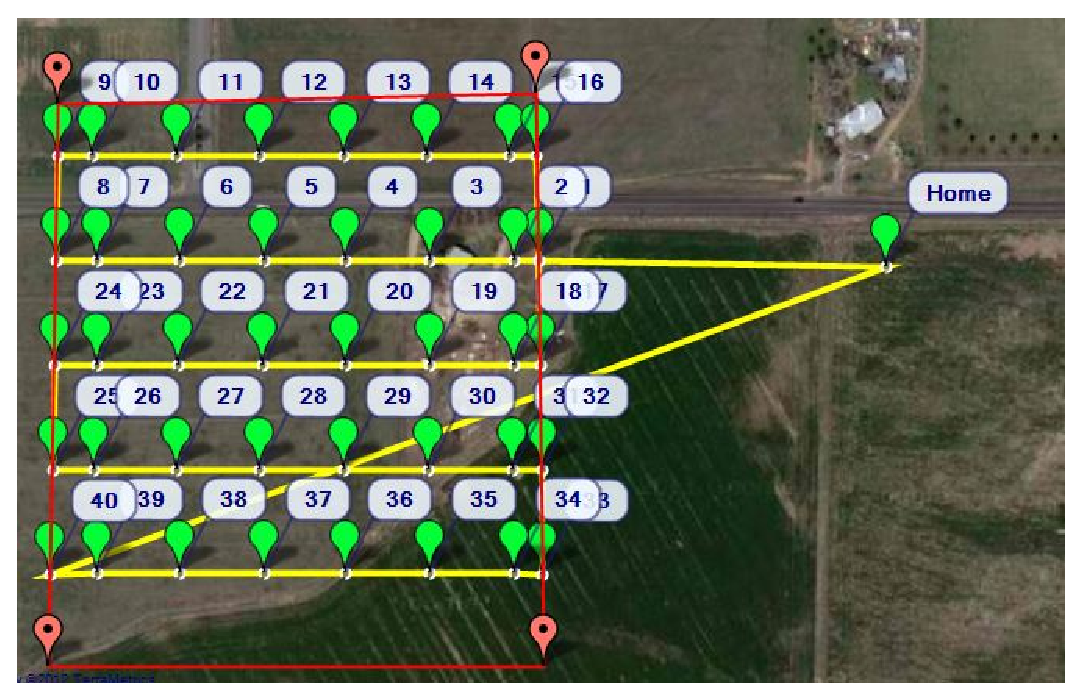
\includegraphics[keepaspectratio=true,scale=0.8]{figuras/esplanada.eps}
    \caption{Simulação feita na Esplanada. Fonte: Software \textit{Mission Planner}}
    \label{fig:esplanada}
\end{figure}

A plataforma a ser utilizado será o Microsoft Windows devido à grande utilização no Serviço Público, 
além de oferecer maior compatibilidade com os recursos utilizados, obedecendo, por exemplo, os requisitos
do sistema de comunicação com o controlador, o Mission Planner. 

\subsubsubsection{Protocolo de erros}
	
Para um funcionamento seguro é necessário ter em mente que podem vir a existir condições adversas as planejadas. Tendo isso em vista foi estabelecido um protocolo de erros para situações que podem vir a ocorrer durante um voo do VANT.

\begin{itemize}
 \item Perda de sinal: Em caso de perda de sinal o VANT deverá retornar a seu ponto de origem imediatamente.
 
 \item Bateria fraca: Ao chegar em 25\% restante de bateria o VANT irá retornar para a central imediatamente.

 \item Perda de potência: Em caso de perda de potência por parte do motor, o VANT procurará um local para pousar imediatamente.

\end{itemize}

\subsubsubsection{Comunicação do usuário com o VANT}
Nessa subseção é tratada a comunicação da central com o VANT e do cidadão com o VANT.
Nessa comunicação alguns passos devem ser seguidos, são eles:

\subsubsubsection{Processo de atendimento adotado}
Mediante análise do sistema de atendimento de urgências e classificação da situação-problema adotado em uma capital brasileira, além de questões de segurança de uso do VANT, identificou-se a necessidade de um protocolo de atendimento para verificar a viabilidade do atendimento pelo VANT ou por uma viatura comum de atendimento de urgência.
Ao receber a solicitação de socorro, o atendente avalia a situação da emergência, como identificação do paciente, localização do chamado e origem e natureza do solicitante. Em posse dessas informações, verifica-se a necessidade e disponibilidade de uma viatura para atendimento solicitado.

% image

É de competência do médico regulador avaliar qual o melhor recurso para o paciente, ou seja, sua decisão poderá ser a de orientar o solicitante a procurar uma unidade de saúde ou, nos casos necessários, enviar ao local uma Unidade de Suporte Básico, com auxiliar de enfermagem e condutor socorrista, ou uma Unidade de Suporte Avançado, a UTI móvel, com médico e enfermeiro.
A atividade do médico regulador envolve o exercício da Telemedicina, que se dá através da gravação contínua das comunicações, do correto preenchimento das fichas


médicas de regulação e do seguimento de protocolos institucionais normatizados que definam os passos e as bases para sua decisão, sempre julgando a necessidade do envio da melhor resposta e do melhor recurso às diversas solicitações. Nos casos em que o médico regulador julgar desnecessário o envio de uma equipe ao local para atendimento às solicitações, o mesmo deve explicar sua decisão e esclarecer ao demandante do socorro quanto a outras medidas a serem adotadas, por meio de orientação ou conselho médico, que permita ao solicitante assumir cuidados ou buscá-los em local definido pelo médico regulador.

Para garantir um funcionamento adequado do modelo de regulação referenciado, algumas tecnologias estão sendo incorporadas à central de regulação médica das urgências como o sistema de rastreamento dos veículos através de GPS (Global Positioning System) e ainda a transmissão de dados para o interior das ambulâncias e vice-versa.
Estas ferramentas oferecem informações que servem para auxiliar na decisão gestora do regulador médico, uma vez que atuam sobre dois dos grandes nós críticos do atendimento pré-hospitalar móvel, a comunicação qualificada com as equipes de atendimento e a diminuição do tempo resposta.

\subsubsubsection{Avaliação multifatorial do grau de urgência}

O grau de urgência é diretamente proporcional à gravidade, à quantidade de recursos necessários para atender o caso e à pressão social presente na cena do atendimento, e inversamente proporcional ao tempo necessário para iniciar o tratamento. Levando-se em conta esta razão matemática, temos a seguinte fórmula.

% image

\begin{description}
  \item[Gravidade] \hfill \\
  É perfeitamente possível quantificar a gravidade do caso pelo telefone, por meio de perguntas objetivas dirigidas diretamente ao paciente ou à pessoa que ligou solicitando ajuda, utilizando uma semiologia que é definida e abordada nos protocolos específicos.
 \item[Tempo] \hfill \\
 Tratamos aqui de utilizar o conhecimento dos intervalos de tempo aceitáveis entre o início dos sintomas e o início do tratamento. Quanto menor o tempo exigido, maior a urgência.
 \item[Recursos necessários] \hfill \\
 Quanto maior for a necessidade de recursos envolvidos no atendimento inicial e no tratamento definitivo, maior será a urgência. Este subfator é o que mais influi na decisão de transferir o paciente.
  \item[Valor Social] \hfill \\
 A pressão social que envolve o atendimento inicial pode muitas vezes justificar o aumento do grau de urgência de um caso simples. Este fator não pode ser negligenciado, pois muitas vezes uma comoção social no local do atendimento pode dificultar a prestação de socorro.
\end{description}

\subsubsubsection{Classificação das urgências}

Com o objetivo de facilitar o estabelecimento de prioridades entre os diferentes casos de urgência, podemos classificar, didaticamente, as solicitações de socorro da seguinte forma:

% image tabela

Como o veículo aéreo não tripulado se direciona apenas para atendimento de casos de extrema urgência com a impossibilidade da chegada de uma Unidade de Atendimento Básico em tem hábil. O VANT pode ser acionado apenas em casos com classificação 1 (um) de urgência, em que o tempo é primordial para atendimento e que haja algum bloqueio da ambulância.

Avaliando a setorização da Central de Atendimento do Serviço Móvel de Urgência, acontecerá a transferência de comunicação para um setor especializado no controle dos VANT’s que se localizará no mesmo local físico que a Central de Atendimento no Batalhão do Corpo de Bombeiros Militar da Esplanada dos Ministérios próximo ao Palácio do Planalto na Esplanada dos Ministérios em Brasília-DF.

O VANT estará posicionado nessa mesma base, em que um técnico colocará o veículo disponível em local aberto, confirmando as corretas informações dos sensores a central. Após a decolagem o veículo será monitorado apenas pelo software e recursos embutidos. A central pode avaliar toda a situação através de sensores, vídeo e áudio, avaliando assim a correta localização e a emergência. 

Após a conferência, o veículo poderá solicitar espaço para pouso seguro, alertando pessoas próximas para continuação do atendimento. Levando o mesmo para perto do local de emergência e posicionando o sensor no dedo indicador do paciente, averiguando a situação do mesmo identificando se o paciente sofre parada cardíaca ou respiratória.

Caso a situação não trate das doenças supracitadas, observa-se a situação por áudio e vídeo, estabelecendo protocolos de primeiros socorros, até a chegada da Unidade Móvel para o atendimento e recolhimento do veículo.

Entretanto, ao verificar a utilidade do VANT em tal atendimento, a comunicação com um terceiro torna-se essencial para continuação do socorro, por meio de áudio e visualização do paciente pela central. De modo que o atendente especializado possa instruir corretamente terceiros no posicionamento dos sensores do desfibrilador ou da bomba respiratória e os demais passos, como afastamento de pessoas do paciente ou o uso devido da bomba respiratória.

No caso do uso do desfibrilador, por ser um aparelho eletrônico portátil e automático que diagnostica as, potencialmente letais, arritmias cardíacas de fibrilação ventricular e taquicardia ventricular em um paciente. Capaz também de trata-las, através da desfibrilação, uma aplicação de corrente elétrica que para a arritmia, fazendo com que o coração retome o ciclo cardíaco normal.

Já no caso de parada respiratória, as instruções para utilização de Respiração Artificial Instrumental serão passadas e observadas pelo atendente da central. De modo a normalizar a ventilação por via aérea.

A central pode solicitar, via áudio, que o terceiro que auxiliou no atendimento aguarde no local até a chegada da viatura a fim de prevenir outros casos.

\subsubsection{Custos}
  
  Para a parte de comunicação o custo calculado trata-se das modificações a serem realizadas no
  \textit{Mission Planner}, essas modificações podem ser vistas no documento de visão que está
  em anexo.
  
  Dadas as modificações necessárias, para a realização das mesmas, foi definido um planejamento, usando o \textit{Scrum} que
  é uma metodologia ágil e que traz conceitos temporais que serão utilizados nas modificações do \textit{Mission Planner}. 
  
  Dentre os conceitos provenientes de \citeonline{scrum} que serão utilizados no projeto temos as seguintes definições:

  \begin{itemize}
  \item \textit{Release} – Entrega das manutenções planejadas. No projeto de manutenção do \textit{Mission Planner} será após um mês do começo das modificações;
  \item \textit{Sprint} – Ciclo menor de tempo. No projeto de manutenção do \textit{Mission Planner}, possuirá duas semanas de duração.
  \end{itemize}

  \textbf{Planejamento}
   \begin{itemize}
      \item 1ª \textit{Sprint}
	\subitem Retirar função de doar para o projeto;
	\subitem Traduzir menus, instruções e comandos;
	\subitem Criar funcionalidades de \textit{login}.	
      \item 2ª \textit{Sprint}
      \subitem Criar funcionalidade de receber dados do paciente.
      \subitem Adicionar funcionalidade de observação por câmera e comunicação;
      \subitem Definir perfis de acesso e configuração.
  \end{itemize}

 \textbf{Cálculo dos custos}
 
 Para definir os custos, foi definido que cada atividade deverá passar por quatro áreas: 
\begin{itemize}
 \item Requisitos;
\item Desenvolvimento;
\item Teste;
\item Implantação.
\end{itemize}

   Foi definido que a fábrica que realizará a manutenção possuirá três funcionários para cada uma das áreas descritas. 
   Foram definidos os seguintes salários (por hora), baseado no site Info Abril\footnotemark para os funcionários dessas áreas:
\footnotetext{http://info.abril.com.br/carreira/salarios/}
\begin{itemize}
   \item Analista de Requisitos – R\$ 91,50
\item Desenvolvedor – R\$ 53,20
\item Analista de Teste –R\$ 58,80
\item Infraestrutura – R\$ 63,00
\end{itemize}

Sendo assim, tendo em mente que serão duas \textit{sprints} de duas semanas cada, 
e que por dia cada funcionário trabalha 8 horas, temos como custo final o valor de R\$ 63960,00,
conforme detalhamento na figura \ref{fig:custos_software}.
 
 \begin{figure}[H]
    \centering
	    \includegraphics[keepaspectratio=true,scale=0.8]{figuras/custos_software.png}
    \caption{Custos de modificações no \texttt{Mission Planner}}
    \label{fig:custos_software}
\end{figure}

Algo que também deve ser levado em conta é que pode vir a existir a necessidade de manutenção, seja esta corretiva ou evolutiva, 
sendo assim deve ser levado em conta um possível gasto extra além do estabelecido.
